\documentclass[../main.tex]{subfiles}
\graphicspath{{\subfix{../images/}}}
\begin{document}
\section*{Term 2 Week 8}
\begin{enumerate}[itemsep=1cm]
    \item 
    \(\int \sqrt{1-x}.\sqrt{x+3}\,dx\)

    \item 
    Solve the system of equations for both \(x\) and \(y\):\\
    $
    \sin{x}\cos{y}=\frac{1}{4}\\
    \sin{y}\cos{x}=\frac{3}{4}
    $
    
    \item
    If \(\arg{(\frac{z-6}{z-2})}=\frac{\pi}{4}\), give the equation of the locus of \(P(x,y)\).
    
    Recall that \(\arg{(z_1z_2)}=\arg{(z_1)}+\arg{(z_2)}\) and \(\arg{\Bigl(\frac{z_1}{z_2}\Bigr)}=\arg{(z_1)}-\arg{(z_2)}\)

    \item
    ABCD is a rectangle. PQ = 3cm and QR = 2cm.

    Find the radius of the third circle.
    
    \begin{figure}[H]
        \centering
        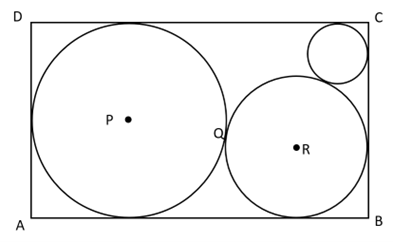
\includegraphics{images/t2w8q4.png}
    \end{figure}
   

    \end{enumerate}

\end{document}